\documentclass[t]{beamer}
\usecolortheme[RGB={0,114,197}]{structure} 
\usetheme{Ilmenau} 
\usepackage{tikz}
\usepackage{multicol}

\title{Software-Ontwerp}
\subtitle{Iteratie 3}
\author{Castel D. - Devlieghere J. - Pante S.}
\institute{KU Leuven}

\begin{document}

\frame{\titlepage} 
\begin{frame}{Inhoud}
\begin{multicols}{2}
\tableofcontents
\end{multicols}
\end{frame}



\section{Inleiding} 

\subsection{Rolverdeling}
\begin{frame}{Rolverdeling}
\begin{multicols}{2}
\tableofcontents[currentsection]
\end{multicols}
\end{frame}

\begin{frame}{Rolverdeling}
Afgelopen iteratie:
\begin{itemize}
	\item Lead Designer: Vincent Reniers
	\item Lead Tester: Jonas Devlieghere
	\item Domain Modeler: Dieter Castel
\end{itemize}
Komende iteratie:
\begin{itemize}
	\item Lead Designer: Stefan Pante
	\item Lead Tester: Dieter Castel
	\item Domain Modeler: Jonas Devlieghere
\end{itemize}
\end{frame}

\subsection{Werkverdeling}

\begin{frame}{Werkverdeling}
\begin{figure}[h!]
	\center
	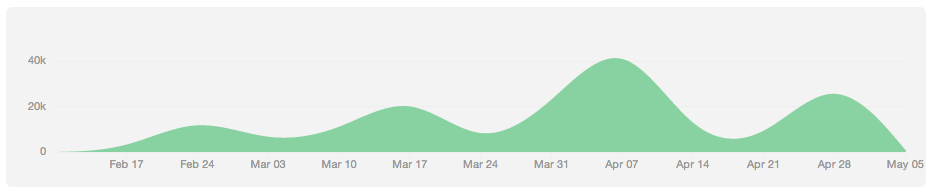
\includegraphics[width= 0.9\linewidth]{img/github.png}
	\caption{Commit history doorheen de iteraties}
\end{figure}

\end{frame}

\section{Tests}

\begin{frame}{Testen}
\begin{multicols}{2}
\tableofcontents[currentsection]
\end{multicols}
\end{frame}

\begin{frame}{Test Coverage}
\begin{figure}[h!]
	\center
	%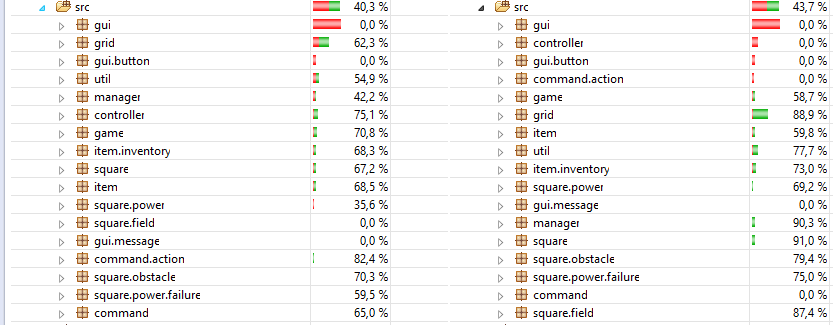
\includegraphics[width= 0.9\linewidth]{img/coverage.png}
	\caption{EclEmma test coverage}
\end{figure}
\end{frame}

\section{Nieuwigheden deze iteratie}

\subsection{Power Failures}

\subsection{Force Fields}
\begin{frame}{Force Fields}
\begin{figure}
	\center
	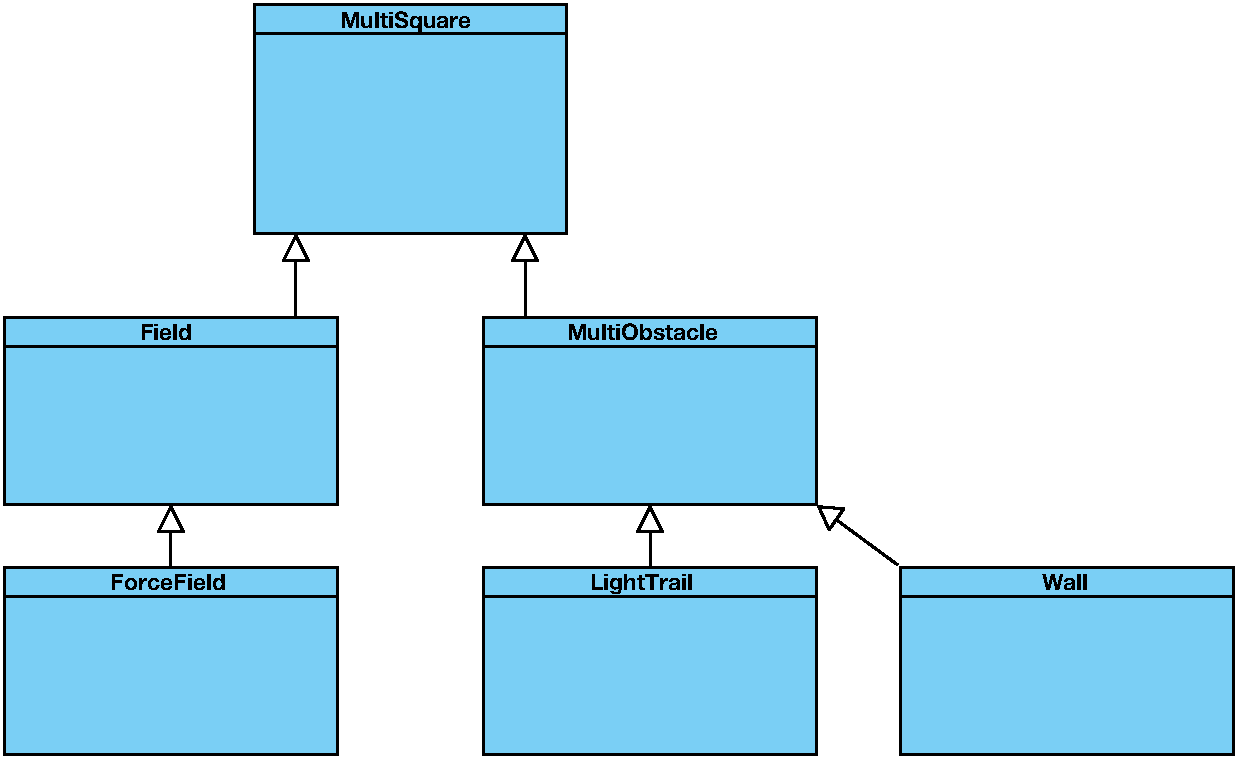
\includegraphics[width= 0.6\linewidth]{img/forcefield.pdf}
	\caption{Fields en Force Fields}
\end{figure}
\end{frame}


\subsubsection{Force Field Generators}
\begin{frame}{Force Field Generators}
\begin{figure}
	\center
	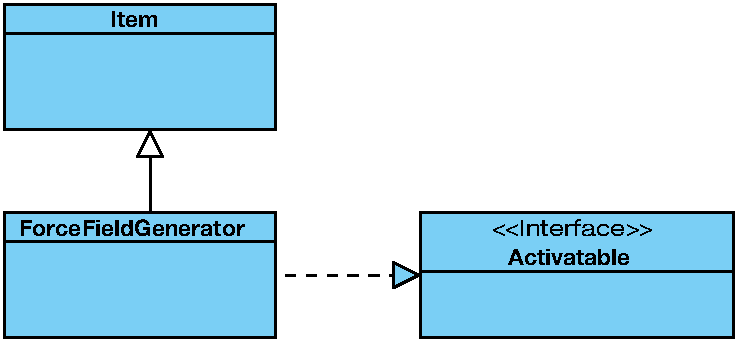
\includegraphics[width= 0.5\linewidth]{img/forcefieldgenerator.pdf}
	\caption{Force Field Generators}
\end{figure}
\begin{itemize}
	\item Force Field Generators zijn \textit{items}
	\item Force Field Generators zijn \textit{activatable}
\end{itemize}
\end{frame}

\subsubsection{Force Field Manager}
\begin{frame}
\begin{multicols}{2}
\begin{figure}
	\center
	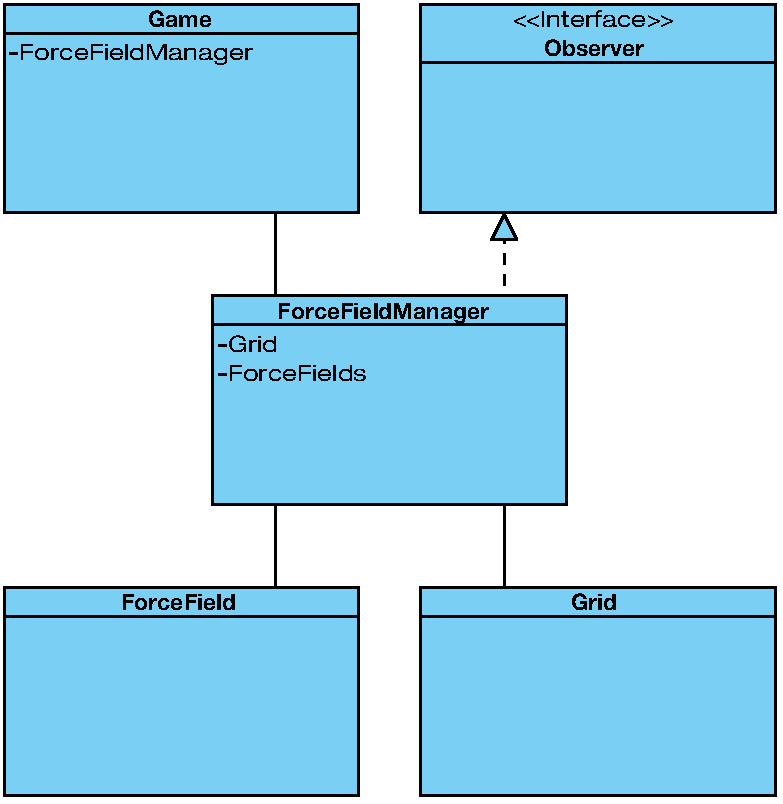
\includegraphics[width= 0.9\linewidth]{img/forcefieldmanager.pdf}
	\caption{Force Field Generators}
\end{figure}

\begin{itemize}
	\item Herkent aan de hand van het Grid welke Force Fields geactiveerd kunnen worden
	\item Gekoppeld met elk force field
	\item Generatoren zijn niet gekoppeld met velden zelf
	\item Observeert acties en schakelt velden aan en uit
\end{itemize}
\end{multicols}
\end{frame}

\subsection{Effect}
\begin{frame}{Effecten}
\begin{itemize}
	\item Effecten zijn geen onderdeel meer van de \textit{commands}
	\item \textbf{Composite Pattern} met \textit{MovableEffect} interface
\end{itemize}
\end{frame}
\subsection{MovableEffect}
\begin{frame}
\begin{figure}
	\center
	%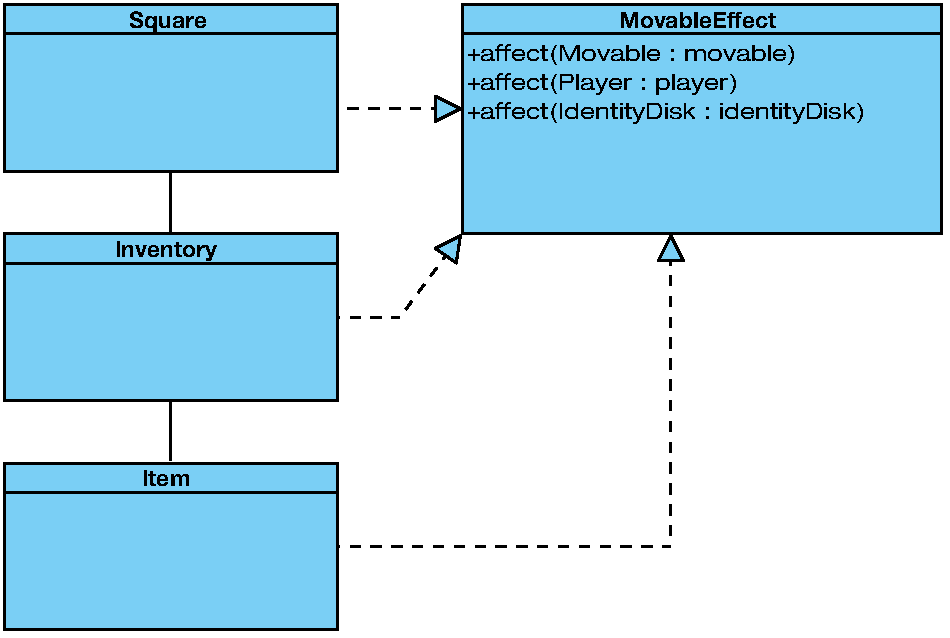
\includegraphics[width= 0.5\linewidth]{img/composite.pdf}
	\caption{Force Field Generators}
\end{figure}
\end{frame}

\section{Aanpassingen}

\subsection{Activatable}
\subsection{Commands}



\section{Slot}
\begin{frame}{Besluit}
\vspace{0.8in}
\begin{center}
Bedankt voor uw aandacht.
\end{center}
\end{frame}

\end{document}
